\documentclass[twoside]{book}

% Packages required by doxygen
\usepackage{fixltx2e}
\usepackage{calc}
\usepackage{doxygen}
\usepackage[export]{adjustbox} % also loads graphicx
\usepackage{graphicx}
\usepackage[utf8]{inputenc}
\usepackage{makeidx}
\usepackage{multicol}
\usepackage{multirow}
\PassOptionsToPackage{warn}{textcomp}
\usepackage{textcomp}
\usepackage[nointegrals]{wasysym}
\usepackage[table]{xcolor}

% Font selection
\usepackage[T1]{fontenc}
\usepackage[scaled=.90]{helvet}
\usepackage{courier}
\usepackage{amssymb}
\usepackage{sectsty}
\renewcommand{\familydefault}{\sfdefault}
\allsectionsfont{%
  \fontseries{bc}\selectfont%
  \color{darkgray}%
}
\renewcommand{\DoxyLabelFont}{%
  \fontseries{bc}\selectfont%
  \color{darkgray}%
}
\newcommand{\+}{\discretionary{\mbox{\scriptsize$\hookleftarrow$}}{}{}}

% Page & text layout
\usepackage{geometry}
\geometry{%
  a4paper,%
  top=2.5cm,%
  bottom=2.5cm,%
  left=2.5cm,%
  right=2.5cm%
}
\tolerance=750
\hfuzz=15pt
\hbadness=750
\setlength{\emergencystretch}{15pt}
\setlength{\parindent}{0cm}
\setlength{\parskip}{0.2cm}
\makeatletter
\renewcommand{\paragraph}{%
  \@startsection{paragraph}{4}{0ex}{-1.0ex}{1.0ex}{%
    \normalfont\normalsize\bfseries\SS@parafont%
  }%
}
\renewcommand{\subparagraph}{%
  \@startsection{subparagraph}{5}{0ex}{-1.0ex}{1.0ex}{%
    \normalfont\normalsize\bfseries\SS@subparafont%
  }%
}
\makeatother

% Headers & footers
\usepackage{fancyhdr}
\pagestyle{fancyplain}
\fancyhead[LE]{\fancyplain{}{\bfseries\thepage}}
\fancyhead[CE]{\fancyplain{}{}}
\fancyhead[RE]{\fancyplain{}{\bfseries\leftmark}}
\fancyhead[LO]{\fancyplain{}{\bfseries\rightmark}}
\fancyhead[CO]{\fancyplain{}{}}
\fancyhead[RO]{\fancyplain{}{\bfseries\thepage}}
\fancyfoot[LE]{\fancyplain{}{}}
\fancyfoot[CE]{\fancyplain{}{}}
\fancyfoot[RE]{\fancyplain{}{\bfseries\scriptsize Generated on Mon Jun 29 2015 20\+:42\+:20 for Easy Defines by Doxygen }}
\fancyfoot[LO]{\fancyplain{}{\bfseries\scriptsize Generated on Mon Jun 29 2015 20\+:42\+:20 for Easy Defines by Doxygen }}
\fancyfoot[CO]{\fancyplain{}{}}
\fancyfoot[RO]{\fancyplain{}{}}
\renewcommand{\footrulewidth}{0.4pt}
\renewcommand{\chaptermark}[1]{%
  \markboth{#1}{}%
}
\renewcommand{\sectionmark}[1]{%
  \markright{\thesection\ #1}%
}

% Indices & bibliography
\usepackage{natbib}
\usepackage[titles]{tocloft}
\setcounter{tocdepth}{3}
\setcounter{secnumdepth}{5}
\makeindex

% Hyperlinks (required, but should be loaded last)
\usepackage{ifpdf}
\ifpdf
  \usepackage[pdftex,pagebackref=true]{hyperref}
\else
  \usepackage[ps2pdf,pagebackref=true]{hyperref}
\fi
\hypersetup{%
  colorlinks=true,%
  linkcolor=blue,%
  citecolor=blue,%
  unicode%
}

% Custom commands
\newcommand{\clearemptydoublepage}{%
  \newpage{\pagestyle{empty}\cleardoublepage}%
}


%===== C O N T E N T S =====

\begin{document}

% Titlepage & ToC
\hypersetup{pageanchor=false,
             bookmarks=true,
             bookmarksnumbered=true,
             pdfencoding=unicode
            }
\pagenumbering{roman}
\begin{titlepage}
\vspace*{7cm}
\begin{center}%
{\Large Easy Defines }\\
\vspace*{1cm}
{\large Generated by Doxygen 1.8.10}\\
\vspace*{0.5cm}
{\small Mon Jun 29 2015 20:42:20}\\
\end{center}
\end{titlepage}
\clearemptydoublepage
\tableofcontents
\clearemptydoublepage
\pagenumbering{arabic}
\hypersetup{pageanchor=true}

%--- Begin generated contents ---
\chapter{Hierarchical Index}
\section{Class Hierarchy}
This inheritance list is sorted roughly, but not completely, alphabetically\+:\begin{DoxyCompactList}
\item \contentsline{section}{Easy\+Define}{\pageref{struct_easy_define}}{}
\item \contentsline{section}{Easy\+Define\+Tools}{\pageref{class_easy_define_tools}}{}
\item Editor\+Window\begin{DoxyCompactList}
\item \contentsline{section}{Easy\+Defines\+Window}{\pageref{class_easy_defines_window}}{}
\end{DoxyCompactList}
\end{DoxyCompactList}

\chapter{Class Index}
\section{Class List}
Here are the classes, structs, unions and interfaces with brief descriptions\+:\begin{DoxyCompactList}
\item\contentsline{section}{\hyperlink{struct_easy_define}{Easy\+Define} \\*Structure used for syncing define data. }{\pageref{struct_easy_define}}{}
\item\contentsline{section}{\hyperlink{class_easy_defines_window}{Easy\+Defines\+Window} \\*Custom window for working with Easy Defines. }{\pageref{class_easy_defines_window}}{}
\item\contentsline{section}{\hyperlink{class_easy_define_tools}{Easy\+Define\+Tools} \\*Tools for basic Easy Define functionality. }{\pageref{class_easy_define_tools}}{}
\end{DoxyCompactList}

\chapter{Class Documentation}
\hypertarget{struct_easy_define}{}\section{Easy\+Define Struct Reference}
\label{struct_easy_define}\index{Easy\+Define@{Easy\+Define}}


Structure used for syncing define data.  


\subsection*{Public Attributes}
\begin{DoxyCompactItemize}
\item 
\hypertarget{struct_easy_define_a9ec78d3aad3051a8125ef646b9e6506c}{}string {\bfseries m\+\_\+define\+Name}\label{struct_easy_define_a9ec78d3aad3051a8125ef646b9e6506c}

\item 
\hypertarget{struct_easy_define_a4fdb61309a73e3a92c7233bf71a0d43c}{}bool {\bfseries m\+\_\+cs\+Active}\label{struct_easy_define_a4fdb61309a73e3a92c7233bf71a0d43c}

\item 
\hypertarget{struct_easy_define_a348436a6ffcf427d84fdb0923a91472e}{}bool {\bfseries m\+\_\+editor\+Active}\label{struct_easy_define_a348436a6ffcf427d84fdb0923a91472e}

\item 
\hypertarget{struct_easy_define_a31989bfb9a97f3d612a639c0d0988765}{}bool {\bfseries m\+\_\+us\+Active}\label{struct_easy_define_a31989bfb9a97f3d612a639c0d0988765}

\end{DoxyCompactItemize}


\subsection{Detailed Description}
Structure used for syncing define data. 



The documentation for this struct was generated from the following file\+:\begin{DoxyCompactItemize}
\item 
Editor/Easy\+Define.\+cs\end{DoxyCompactItemize}

\hypertarget{class_easy_defines_window}{}\section{Easy\+Defines\+Window Class Reference}
\label{class_easy_defines_window}\index{Easy\+Defines\+Window@{Easy\+Defines\+Window}}


Custom window for working with Easy Defines.  


Inheritance diagram for Easy\+Defines\+Window\+:\begin{figure}[H]
\begin{center}
\leavevmode
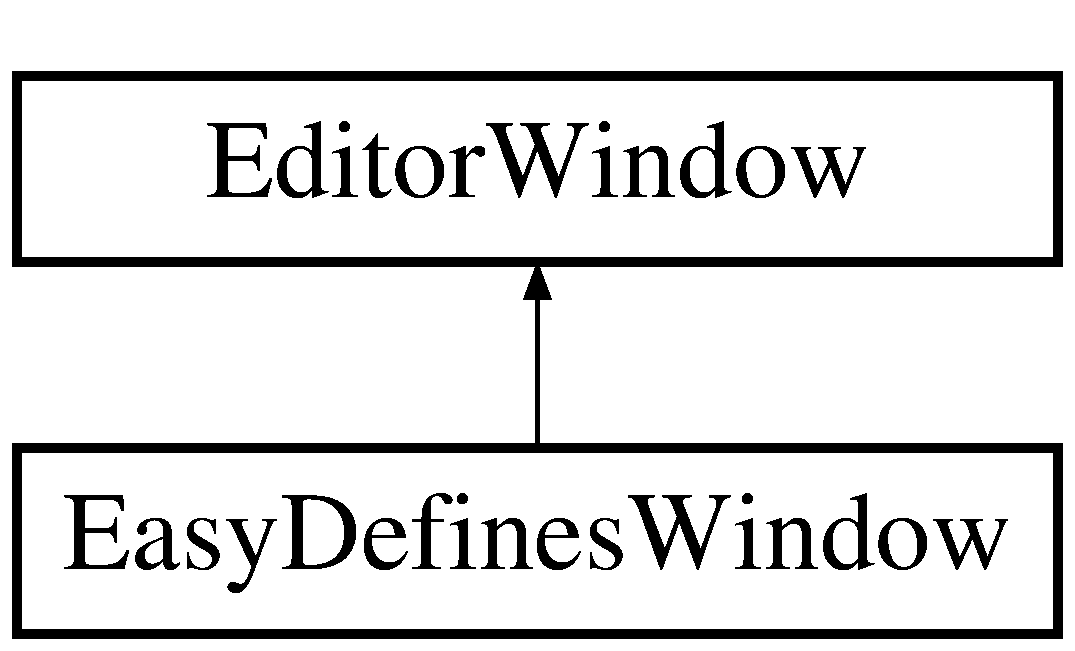
\includegraphics[height=2.000000cm]{class_easy_defines_window}
\end{center}
\end{figure}
\subsection*{Static Public Member Functions}
\begin{DoxyCompactItemize}
\item 
static void \hyperlink{class_easy_defines_window_ae50ce9c23637190a5d7657dbeac681ff}{Show\+Window} ()
\begin{DoxyCompactList}\small\item\em Shows the Easy Define window. \end{DoxyCompactList}\end{DoxyCompactItemize}


\subsection{Detailed Description}
Custom window for working with Easy Defines. 



\subsection{Member Function Documentation}
\hypertarget{class_easy_defines_window_ae50ce9c23637190a5d7657dbeac681ff}{}\index{Easy\+Defines\+Window@{Easy\+Defines\+Window}!Show\+Window@{Show\+Window}}
\index{Show\+Window@{Show\+Window}!Easy\+Defines\+Window@{Easy\+Defines\+Window}}
\subsubsection[{Show\+Window()}]{\setlength{\rightskip}{0pt plus 5cm}static void Easy\+Defines\+Window.\+Show\+Window (
\begin{DoxyParamCaption}
{}
\end{DoxyParamCaption}
)\hspace{0.3cm}{\ttfamily [static]}}\label{class_easy_defines_window_ae50ce9c23637190a5d7657dbeac681ff}


Shows the Easy Define window. 



The documentation for this class was generated from the following file\+:\begin{DoxyCompactItemize}
\item 
Editor/Easy\+Defines\+Window.\+cs\end{DoxyCompactItemize}

\hypertarget{class_easy_define_tools}{}\section{Easy\+Define\+Tools Class Reference}
\label{class_easy_define_tools}\index{Easy\+Define\+Tools@{Easy\+Define\+Tools}}


Tools for basic Easy Define functionality.  


\subsection*{Public Types}
\begin{DoxyCompactItemize}
\item 
\hypertarget{class_easy_define_tools_a2e974776840fb71bf36a91696e28b3ec}{}enum {\bfseries Define\+Type} \{ {\bfseries C\+\_\+\+S\+H\+A\+R\+P} = 1, 
{\bfseries C\+\_\+\+S\+H\+A\+R\+P\+\_\+\+E\+D\+I\+T\+O\+R} = 2, 
{\bfseries U\+N\+I\+T\+Y\+S\+C\+R\+I\+P\+T} = 4
 \}\label{class_easy_define_tools_a2e974776840fb71bf36a91696e28b3ec}

\end{DoxyCompactItemize}
\subsection*{Static Public Member Functions}
\begin{DoxyCompactItemize}
\item 
static void \hyperlink{class_easy_define_tools_a7f1ece2d15f626ab536832217bc31c07}{Force\+Recompile} ()
\begin{DoxyCompactList}\small\item\em Forces a recompile of scripts. \end{DoxyCompactList}\item 
static List$<$ \hyperlink{struct_easy_define}{Easy\+Define} $>$ \hyperlink{class_easy_define_tools_a7e60d8153201ed5e2aeab1f462927590}{Get\+All\+Defines} ()
\begin{DoxyCompactList}\small\item\em Gets all defines. \end{DoxyCompactList}\item 
static void \hyperlink{class_easy_define_tools_ad1d68b0ebdf0a0a0cfcb8ef6d0fba90f}{Sync\+Easy\+Defines\+To\+Sync\+File} ()
\begin{DoxyCompactList}\small\item\em Syncs the easy defines to sync file. \end{DoxyCompactList}\item 
static void \hyperlink{class_easy_define_tools_a7e4a5e6a6890cd324a51dfbc1bd33b3f}{Sync\+Defines\+To\+R\+S\+P} ()
\begin{DoxyCompactList}\small\item\em Syncs the defines to the appropriate R\+S\+P files. \end{DoxyCompactList}\end{DoxyCompactItemize}
\subsection*{Static Public Attributes}
\begin{DoxyCompactItemize}
\item 
\hypertarget{class_easy_define_tools_a7f30cf451ac200a043db23ae3d52bf5b}{}static readonly string {\bfseries S\+Y\+N\+C\+\_\+\+F\+I\+L\+E\+\_\+\+L\+O\+C\+A\+T\+I\+O\+N} = \char`\"{}/Easy\+Defines/Easy\+Defines.\+txt\char`\"{}\label{class_easy_define_tools_a7f30cf451ac200a043db23ae3d52bf5b}

\item 
\hypertarget{class_easy_define_tools_ab531cc79bd1527d96258f30a48e76e0c}{}static readonly string {\bfseries I\+N\+A\+C\+T\+I\+V\+E\+\_\+\+D\+E\+F\+I\+N\+E\+\_\+\+P\+R\+E\+F\+I\+X} = \char`\"{}\+:0\+:0\+:0\char`\"{}\label{class_easy_define_tools_ab531cc79bd1527d96258f30a48e76e0c}

\item 
\hypertarget{class_easy_define_tools_a8565818e56b3af1b5222fd8ff257f9ec}{}static readonly string {\bfseries F\+U\+L\+L\+\_\+\+D\+E\+F\+I\+N\+E\+\_\+\+T\+E\+X\+T} = \char`\"{}\{0\}\+:\{1\}\+:\{2\}\+:\{3\}\+:\{4\}\char`\"{}\label{class_easy_define_tools_a8565818e56b3af1b5222fd8ff257f9ec}

\end{DoxyCompactItemize}


\subsection{Detailed Description}
Tools for basic Easy Define functionality. 



\subsection{Member Function Documentation}
\hypertarget{class_easy_define_tools_a7f1ece2d15f626ab536832217bc31c07}{}\index{Easy\+Define\+Tools@{Easy\+Define\+Tools}!Force\+Recompile@{Force\+Recompile}}
\index{Force\+Recompile@{Force\+Recompile}!Easy\+Define\+Tools@{Easy\+Define\+Tools}}
\subsubsection[{Force\+Recompile()}]{\setlength{\rightskip}{0pt plus 5cm}static void Easy\+Define\+Tools.\+Force\+Recompile (
\begin{DoxyParamCaption}
{}
\end{DoxyParamCaption}
)\hspace{0.3cm}{\ttfamily [static]}}\label{class_easy_define_tools_a7f1ece2d15f626ab536832217bc31c07}


Forces a recompile of scripts. 

\hypertarget{class_easy_define_tools_a7e60d8153201ed5e2aeab1f462927590}{}\index{Easy\+Define\+Tools@{Easy\+Define\+Tools}!Get\+All\+Defines@{Get\+All\+Defines}}
\index{Get\+All\+Defines@{Get\+All\+Defines}!Easy\+Define\+Tools@{Easy\+Define\+Tools}}
\subsubsection[{Get\+All\+Defines()}]{\setlength{\rightskip}{0pt plus 5cm}static List$<${\bf Easy\+Define}$>$ Easy\+Define\+Tools.\+Get\+All\+Defines (
\begin{DoxyParamCaption}
{}
\end{DoxyParamCaption}
)\hspace{0.3cm}{\ttfamily [static]}}\label{class_easy_define_tools_a7e60d8153201ed5e2aeab1f462927590}


Gets all defines. 

\begin{DoxyReturn}{Returns}
The all defines.
\end{DoxyReturn}
\hypertarget{class_easy_define_tools_a7e4a5e6a6890cd324a51dfbc1bd33b3f}{}\index{Easy\+Define\+Tools@{Easy\+Define\+Tools}!Sync\+Defines\+To\+R\+S\+P@{Sync\+Defines\+To\+R\+S\+P}}
\index{Sync\+Defines\+To\+R\+S\+P@{Sync\+Defines\+To\+R\+S\+P}!Easy\+Define\+Tools@{Easy\+Define\+Tools}}
\subsubsection[{Sync\+Defines\+To\+R\+S\+P()}]{\setlength{\rightskip}{0pt plus 5cm}static void Easy\+Define\+Tools.\+Sync\+Defines\+To\+R\+S\+P (
\begin{DoxyParamCaption}
{}
\end{DoxyParamCaption}
)\hspace{0.3cm}{\ttfamily [static]}}\label{class_easy_define_tools_a7e4a5e6a6890cd324a51dfbc1bd33b3f}


Syncs the defines to the appropriate R\+S\+P files. 

\hypertarget{class_easy_define_tools_ad1d68b0ebdf0a0a0cfcb8ef6d0fba90f}{}\index{Easy\+Define\+Tools@{Easy\+Define\+Tools}!Sync\+Easy\+Defines\+To\+Sync\+File@{Sync\+Easy\+Defines\+To\+Sync\+File}}
\index{Sync\+Easy\+Defines\+To\+Sync\+File@{Sync\+Easy\+Defines\+To\+Sync\+File}!Easy\+Define\+Tools@{Easy\+Define\+Tools}}
\subsubsection[{Sync\+Easy\+Defines\+To\+Sync\+File()}]{\setlength{\rightskip}{0pt plus 5cm}static void Easy\+Define\+Tools.\+Sync\+Easy\+Defines\+To\+Sync\+File (
\begin{DoxyParamCaption}
{}
\end{DoxyParamCaption}
)\hspace{0.3cm}{\ttfamily [static]}}\label{class_easy_define_tools_ad1d68b0ebdf0a0a0cfcb8ef6d0fba90f}


Syncs the easy defines to sync file. 



The documentation for this class was generated from the following file\+:\begin{DoxyCompactItemize}
\item 
Editor/Easy\+Define\+Tools.\+cs\end{DoxyCompactItemize}

%--- End generated contents ---

% Index
\backmatter
\newpage
\phantomsection
\clearemptydoublepage
\addcontentsline{toc}{chapter}{Index}
\printindex

\end{document}
